\chapter{Программа “Spectral Analyzer PK-4”}
\label{cha:ch_4}
\section{Актуальность программы}
В ходе данной работы был создан веб-сервис “Spectral~Analyzer~PK-4”, название которого состоит из двух частей:
первая часть (“Spectral~Analyzer”) обозначает главную задачу сервиса - спектральный анализ, а вторая часть говорит
о том, что анализ осуществляется на данных, полученных с исследуемой в текущей работе экспериментальной установки
“Плазменный~кристалл-4” (PK-4). Какие задачи решает “Spectral~Analyzer~PK-4”?

Наиболее важная задача - это, собственно, обработка огромного количества спектральной информации, поступающей с борта МКС
Российско-европейской Космической Аппаратуры “Плазменный~кристалл-4”. Поскольку спектральные данные представляют собой
довольно сложную, но упорядоченную структуру данных (см раздел \ref{cha:ch_3_4}), то ручная обработка и
графическое построение даже одного спектра является времязатратной и трудоёмкой задачей: необходимо ориентироваться
в текстовых логах, а также владеть навыками работы, как минимум, с двумя программами одновременно~-~Origin и Exсel.
У умелого пользователя данных программ (при большом желании) получится построить один спектр не быстрее, чем за 5~мин.
Так как в одном эксперименте возможность встретить более 1000~спектров - обычное явление, то даже таких умений становится недостаточно.

Далее, ожидается, что веб-сервис даст инструмент первичной спектральной обработки: полиномиальная калибровка длин волн,
вычитание и усреднение шумового фона, автоопределение пиков спектральных линий, усреднение идентичных спектров при одних
и тех же параметрах и др.

Мотивационный момент, в будущем данный веб-сервис может быть полезен для подготовки датасетов для применения алгоритмов
машинного обучения.

Поскольку в данной работе разработана и применена методика поиска относительного изменения электронной температуры на основе
отношения интенсивностей спектральных линий, то для “Spectral~Analyzer~PK-4” ставится задача рассчета отношений интенсивностей
спектральных линий в зависимости от энергии верхнего уровня.

Еще один мотивационный момент, данный веб-сервис потенциально дает возможность взаимодействовать
с немецкими коллегами по космической аппаратуре ПК-4.

Таким образом, было решено создать автоматизированное компьютеризированное программное обеспечение для решения данных проблем.

\section{Требования к программе}
Чтобы было не только удобно и практично пользоваться и совершенствовать программу, но и для достижения решения
поставленных задач, были выдвинуты определенные требования к программе.

Во первых, программа должна обладать свойством кроссплатформенности, т.е. независимо от типа операционной
системы она должна работать корректно. Конкретнее, должна быть возможность работы под следующими операционными
системами: Windows~XP - Windows~10, MacOs, Linux с графической оболочкой.

Во вторых, программа должна иметь возможность сохранения ключевых состояний процесса обработки данных,
а также максимально безболезненно передавать прогресс между пользователями.

Далее, программа должна уметь в автоматическом режиме загружать и парсить текстовые спектральные данные
(эксперименты), а также отображать список уже загруженных экспериментов.

Следующий важнейший аспект - это умение динамически отображать более 1000~спектральных графиков в одном
рабочем окне, отображать метаинформацию по текущему спектру.

Для обработки спектров необходимо учитывать фоновое излучение, поэтому программа должна иметь возможность по
выбранным пользователем номерам спектров усреднять их интенсивности, а также вычитать из всех спектров текущего эксперимента.

Не менее важный аспект - это возможность настроить калибровку спектра по длине волны на основе вводимой пользователем полиномиальной функции.

Далее, для поиска отношений интенсивностей необходимо на основе откалиброванных незашумленных спектров сохранять
усредненные спектры-заготовки с учётом среднеквадратичных погрешностей, также необходимо отображать
список уже сохранённых усредненных спектров.

В силу того, что используемый спектрометр “OceanOptics~USB2000+” имеет невысокую разрешающую
способность (см раздел \ref{cha:ch_3_4}), то для корректного поиска отношений интенсивностей
необходимо учитывать наложения линий друг на друга с помощью аппаратной функции спектрометра,
т.е. следующее требование к программе: она должна уметь на основе полиномиального приближения аппаратной
функции учитывать перекрытия рядом стоящих линий с учетом погрешностей.

В данной работе особый интерес представляет зависимость отношения интенсивностей определенных линий от энергии
возбужденного состояния, для этого программа должна иметь библиотеку спектральных линий, а также функционал
по выбору набора линий при построении данной зависимости.

Таким образом, мы перечислили основные требования к программе, а сейчас разберем стек технологий,
который был изучен для достижения данных целей (см.~рис.~\ref{fig:it_tech}).
\begin{figure}[t]
  \centering
  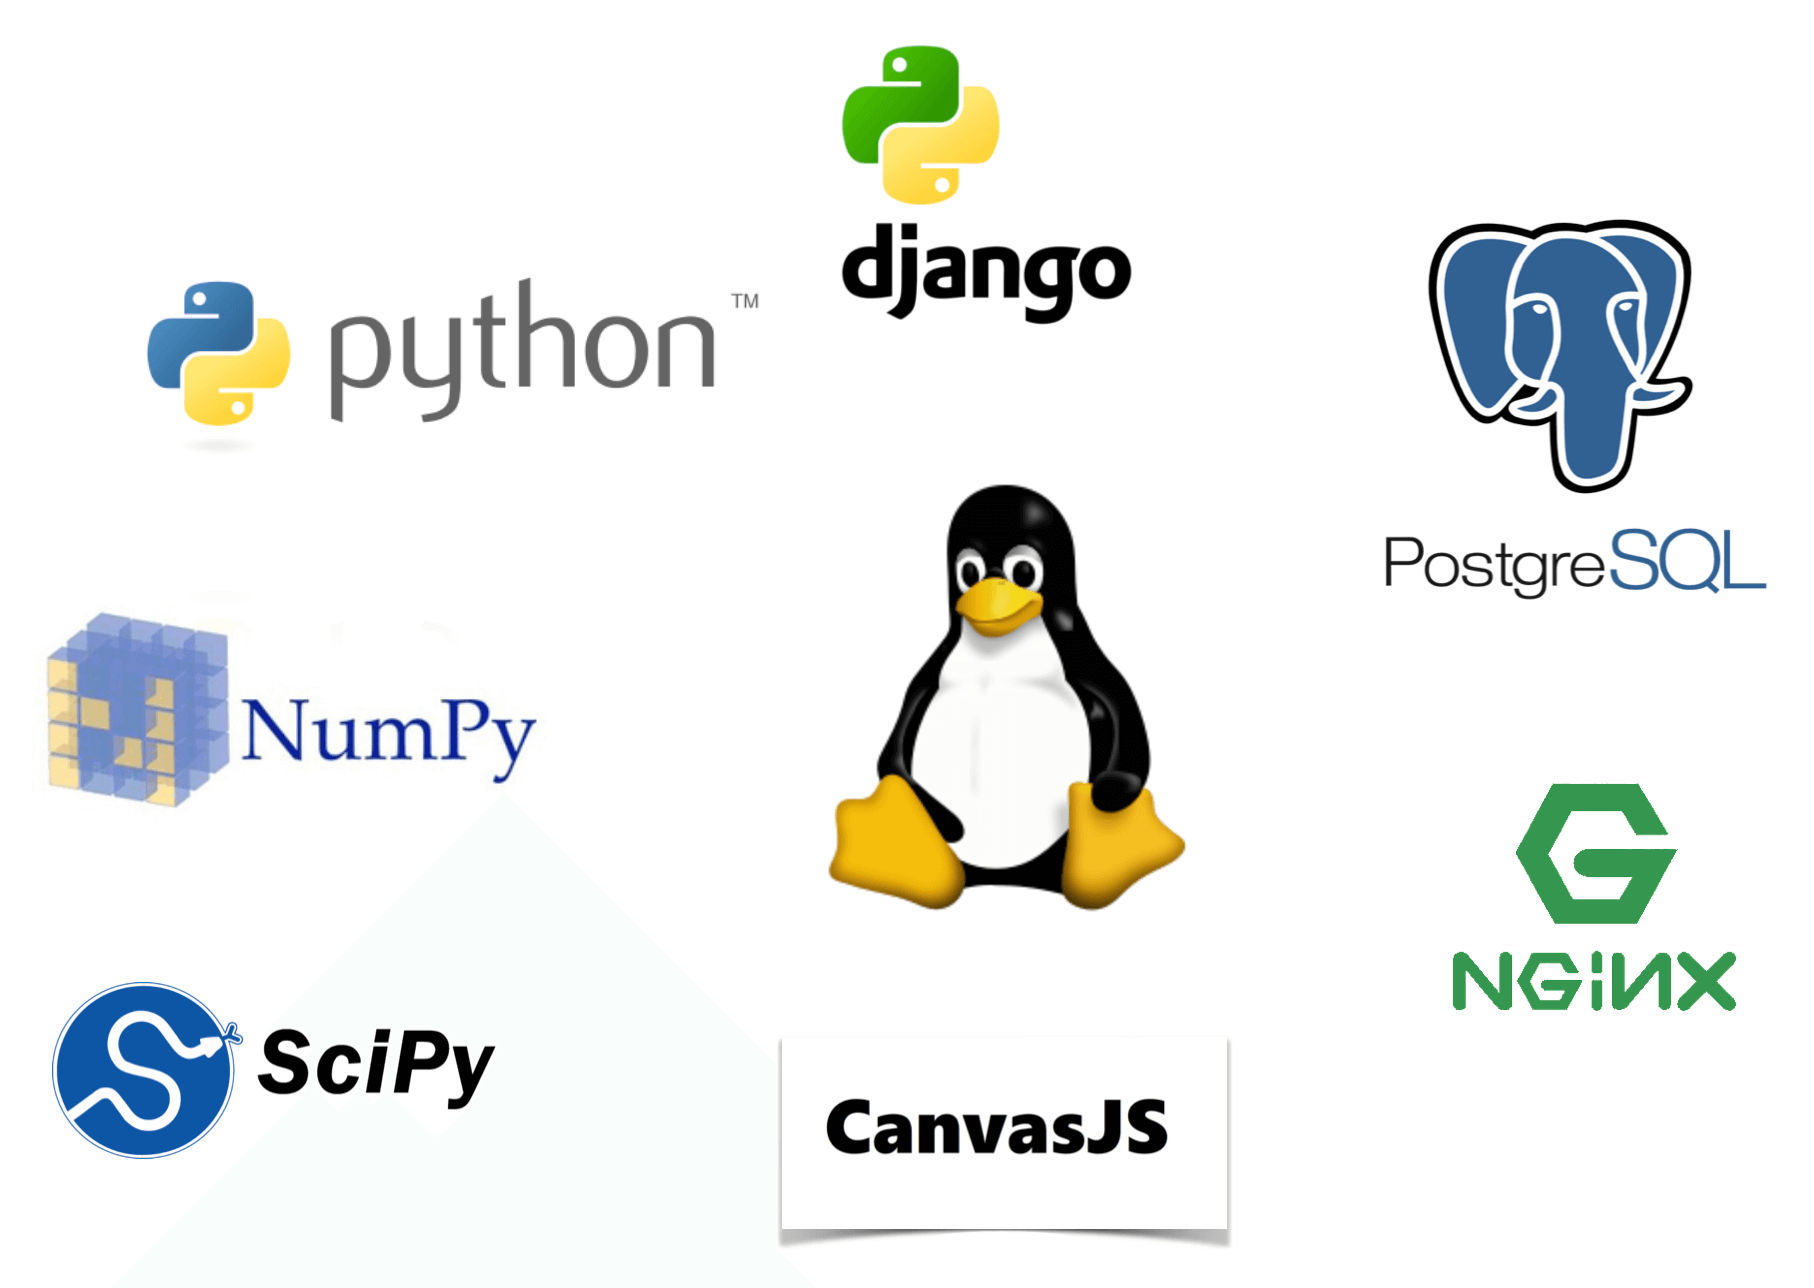
\includegraphics[width=12cm]{figures/it_tech}
  \caption{Изображены логотипы изученных IT-технологий, которые использовались для создания веб-сервиса “Spectral~Analyzer~PK-4”}
  \label{fig:it_tech}
\end{figure}

\section{Стек изученных технологий}
Первый прототип программы был написан традиционным образом на языке C\#, который непременно предполагает
стандартную установку под Windows и работу с программой, как с ПО для данной операционной системы.
В данном варианте было реализовано лишь около 20\% необходимого функционала, но при этом возникли большие трудности
с передачей программы научному руководителю из-за несовместимости версий Windows~7 и XP.

Для решения проблем кроссплатформенности и передачи данных между пользователями было решено создать веб-сервис,
который работает в обычном браузере, поскольку почти каждая операционная система с графической оболочкой
поддерживает большинство современных браузеров.

Django (Джанго)~--~свободный фреймворк для веб-приложений на языке Python, использующий шаблон проектирования MVC.
Проект поддерживается организацией Django Software Foundation \cite{Django}. Джанго имеет удобную гибкую
внутреннюю архитектуру, которая позволяет разработчикам, при достаточных знаниях, выполнять огромный спектр задач
из области веб-программирования. Перечислять все возможности данного фреймворка нет необходимости, подчеркнем лишь те,
что были использованы для решения поставленных задач.

Джанго имеет свою стандартизированную ORM, которая поддерживает транзакции. ORM (англ. Object-Relational Mapping,
рус. объектно-реляционное отображение или преобразование)~--~это некая оболочка над базой данных, которая позволяет
использовать функционал базы данных с помощью объектно-ориентированного языка программирования, в данном случае с помощью Python.

Далее, в Джанго есть система маршрутизации урлов, которая позволяет настраивать POST и GET запросы на основе регулярных выражений,
что очень удобно: в Python есть хорошо известный и понятный встроенный модуль “re”, который почти ничем не отличается по синтаксису.

В Джанго предусмотрена возможность применения криптографически шифрованных Cookie и CSRF-токенов для защиты POST
запросов к серверу: например, для аутентификации пользователя, для любого изменения и некоторых запросов к информации сервера.
Это дает довольно хорошую защиту от мошеннических и хакерских атак.

PostgreSQL~--~свободная объектно-реляционная система управления базами данных, разработанная в Калифорнийском
университете на факультете компьютерных наук в Беркли \cite{PostgreSQL}. PostgreSQL поддерживает большой набор встроенных типов данных:
\begin{itemize}
\item численные типы;
\item двоичные типы;
\item типы «дата/время»;
\item булев тип;
\item перечисление;
\item геометрические примитивы;
\item UUID-идентификатор;
\item XML-данные;
\item массивы;
\item JSON;
\item идентификаторы объектов БД;
\item псевдотипы;
\end{itemize}

NumPy является основным пакетом для научных вычислений в Python, которая поддерживает
многомерные массивы (в~т.ч.~матрицы), а также предоставляет прекрасно оптимизированные высокоуровневые методы для работы с ними,
включая математические, логические, манипуляции с размерностью, сортировку, отбор, ввод-вывод, дискретные преобразования Фурье,
основную линейную алгебру, основные статистические операции, случайное моделирование и многое другое \cite{Numpy}.
Исходный код NumPy находится в открытом доступе.

SciPy — библиотека для языка программирования Python с открытым исходным кодом, предназначенная для выполнения научных и
инженерных расчётов \cite{Scipy}. Возможности:
\begin{itemize}
\item поиск минимумов и максимумов функций;
\item вычисление интегралов функций;
\item поддержка специальных функций;
\item обработка сигналов;
\item обработка изображений;
\item работа с генетическими алгоритмами;
\item решение обыкновенных дифференциальных уравнений;
\end{itemize}

CanvasJS - библиотека для языка программирования JavaScript, которая предоставляет API для работы с диаграммами и графиками
в веб-проектах. Для студентов и некоммерческого использования лицензия предоставляется бесплатно. Основные преимущества:
\begin{itemize}
\item простой API;
\item высокая производительность;
\item 30 типов диаграмм;
\item хорошая документация;
\item поддержка браузеров Chrome, Firefox, Safari, IE8+;
\end{itemize}

При создании веб-сервиса "Spectral~Analyzer~PK-4" использовались следующие версии библиотек:
\begin{itemize}
\item django==2.0;
\item psycopg2==2.7.1;
\item numpy==1.14.2;
\item django-debug-toolbar==1.8;
\item scipy==1.0.1;
\item python-dateutil==2.6.1;
\item canvas-js==2.1
\end{itemize}

\section{Описание функционала}

